% =====================================================================
%  EPD-SDIA-4112 -- Statistique Bayesienne -- Master 1 SDIA
%  CHAPITRE 2 : Distributions a priori et a posteriori
%  Fichier B : sections 2.2 (choisir un a priori) et 2.3 (controles predictifs)
% =====================================================================

% ---------------------------------------------------------------- 1
% [suite]
\begin{frame}{2.2 — Qu'est-ce qu'un a priori défendable ?}
% [rogna]
\small
\begin{kbox}[Les trois niveaux d'information]
\begin{itemize}
  \item \textbf{Non informatif} — on refuse d'injecter du contenu : uniforme, Jeffreys,
        a priori de référence. Objectif : laisser les données décider.
  \item \textbf{Faiblement informatif} — on borne l'\emph{échelle} plausible sans
        affirmer de valeur centrale : $\N(0,1)$ sur une variable standardisée.
        C'est la recommandation moderne (Gelman et al.).
  \item \textbf{Informatif} — on encode une connaissance substantielle
        (essai antérieur, contrainte physique, avis d'expert).
\end{itemize}
\end{kbox}
\vspace{1mm}
\end{frame}

% [suite]
\begin{frame}{2.2 — Qu'est-ce qu'un a priori défendable ? (suite)}
\begin{columns}[t]
\begin{column}{0.55\textwidth}
\begin{ebox}[Le même chiffre, trois lectures]
La « taille » d'un prior Beta se lit dans $a+b$, le nombre d'observations virtuelles
(\textbf{calculé} dans \file{src/fig\_ch2c\_poids.py}) :
\begin{center}
\begin{tabular}{@{}lcc@{}}
\toprule
\textbf{Prior} & $a+b$ & \textbf{obs. virtuelles} \\
\midrule
Beta$(1,1)$ & 2 & 0 \\
Beta$(2,2)$ & 4 & 2 \\
Beta$(5,3)$ & 8 & 6 \\
Beta$(1{,}3;50)$ & 51,3 & 49,3 \\
Beta$(50,50)$ & 100 & \textbf{98} \\
\bottomrule
\end{tabular}
\end{center}
\end{ebox}
\end{column}
\begin{column}{0.42\textwidth}
\begin{wbox}[La question à poser à chaque fois]
« Si j'avais \textbf{98} observations et qu'elles étaient toutes dans ce sens,
écrirais-je la même chose ? » Si la réponse est non, le prior est trop fort.
Le vérifier : face aux 23 vols de Challenger, Beta$(50,50)$ pèse
$w = \frac{100}{100+23} = 0{,}813$.
\end{wbox}
\end{column}
\end{columns}
\end{frame}

% ---------------------------------------------------------------- 2
\begin{frame}{Boîte à outils : six façons d'écrire un a priori}
\centering
\renewcommand{\arraystretch}{1.25}
\small
\footnotesize\scriptsize\begin{tabular}{@{}p{2.5cm}p{3.9cm}p{1.7cm}p{3.4cm}@{}}
\toprule
\textbf{A priori} & \textbf{Définition} & \textbf{Propre ?} & \textbf{Quand l'utiliser} \\
\midrule
Uniforme & $p(\theta) \propto 1$ sur un domaine borné & oui & proportion ou taux
naturellement borné \\[1mm]
Uniforme sur $\log\theta$ & $p(\theta) \propto 1/\theta$ & non & paramètre d'échelle
positif \\[1mm]
Jeffreys & $p(\theta) \propto \sqrt{\det I(\theta)}$ & non & invariance par
reparamétrisation \\[1mm]
Référence & maximise l'information attendue & non & comparaison objective de
modèles \\[1mm]
Faiblement informatif & centré en 0, échelle fixée & oui & régression, modèles
hiérarchiques \\[1mm]
Informatif & élicitation structurée (expertise) & oui & réplication, données
rares \\[1mm]
\bottomrule
\end{tabular}
\vspace{2mm}
\begin{tcolorbox}[colback=byPurple!6,colframe=byPurple,arc=2mm,width=.94\textwidth]
\small\centering
\textbf{Aucun de ces choix n'est « neutre »} : chacun est une décision scientifique,
et c'est pour cela qu'elle doit être écrite dans le rapport d'analyse.
(Le \emph{power prior} de la section 2.4 est un traitement du \emph{désaccord} entre
données passées et présentes.)
\end{tcolorbox}
\end{frame}

% ---------------------------------------------------------------- 3
\begin{frame}{Le prior de Jeffreys : l'invariance comme principe}
% [rogna]
\footnotesize
\begin{columns}[t]
\begin{column}{0.50\textwidth}
\begin{kbox}[Deux lignes de mathématiques]
$I(\theta)$ est l'information de Fisher d'une observation :
\[
I(\theta) = -\,\E\!\left[\frac{\partial^2 \log p(y \given \theta)}{\partial \theta^2}\right],
\qquad p_{\text{Jeffreys}}(\theta) \propto \sqrt{\det I(\theta)}
\]
Cette règle est \textbf{invariante} : elle donne le même en prior pour $\lambda$ et
$1/\lambda$, ce que ne fait \emph{jamais} l'uniforme.
\end{kbox}
\begin{ebox}[Trois cas calculés dans le cours]
\begin{itemize}
  \item Binomiale : $I(p) = \frac{1}{p(1-p)} \Rightarrow \mathrm{Beta}(1/2, 1/2)$
  \item Poisson : $I(\lambda) = 1/\lambda \Rightarrow \mathrm{Gamma}(1/2, 0)$ (impropre)
  \item Normale, $\mu$ inconnue, $\sigma$ connu : $I(\mu) = 1/\sigma^2 \Rightarrow$
        \textbf{uniforme} (donc impropre si $\mu \in \R$)
\end{itemize}
\end{ebox}
\end{column}
\begin{column}{0.47\textwidth}
\begin{solbox}[Vérification numérique exécutée]
Sur une grille de $20\,001$ valeurs de $p$ :
\[
\begin{aligned}
\max_p\Bigl|\frac{\sqrt{I(p)}}{\max\sqrt{I}}
&- \frac{\text{noyau Beta}(1/2,1/2)}{\max}\Bigr|\\[1mm]
&= 1{,}67 \cdot 10^{-16}
\end{aligned}
\]
c'est-à-dire une identité exacte, à l'erreur machine près.\\
$B(1/2, 1/2) = \pi = 3{,}141593$ (écart numérique avec $\pi$ : $4{,}4 \cdot 10^{-16}$).
\end{solbox}
\begin{wbox}[Le prix à payer]
Jeffreys \textbf{favorise les extrêmes} : $P(p < 0{,}1) = 0{,}2048$ pour
Beta$(0{,}5;0{,}5)$ contre $0{,}1000$ pour l'uniforme. Ce n'est pas de l'ignorance,
c'est une information (les paramètres proches de la frontière sont plus « vrais »
sous reparamétrisation).
\end{wbox}
\end{column}
\end{columns}
\end{frame}

% ---------------------------------------------------------------- 4
\begin{frame}{Jeffreys au banc d'essai : les petits échantillons}
\begin{center}
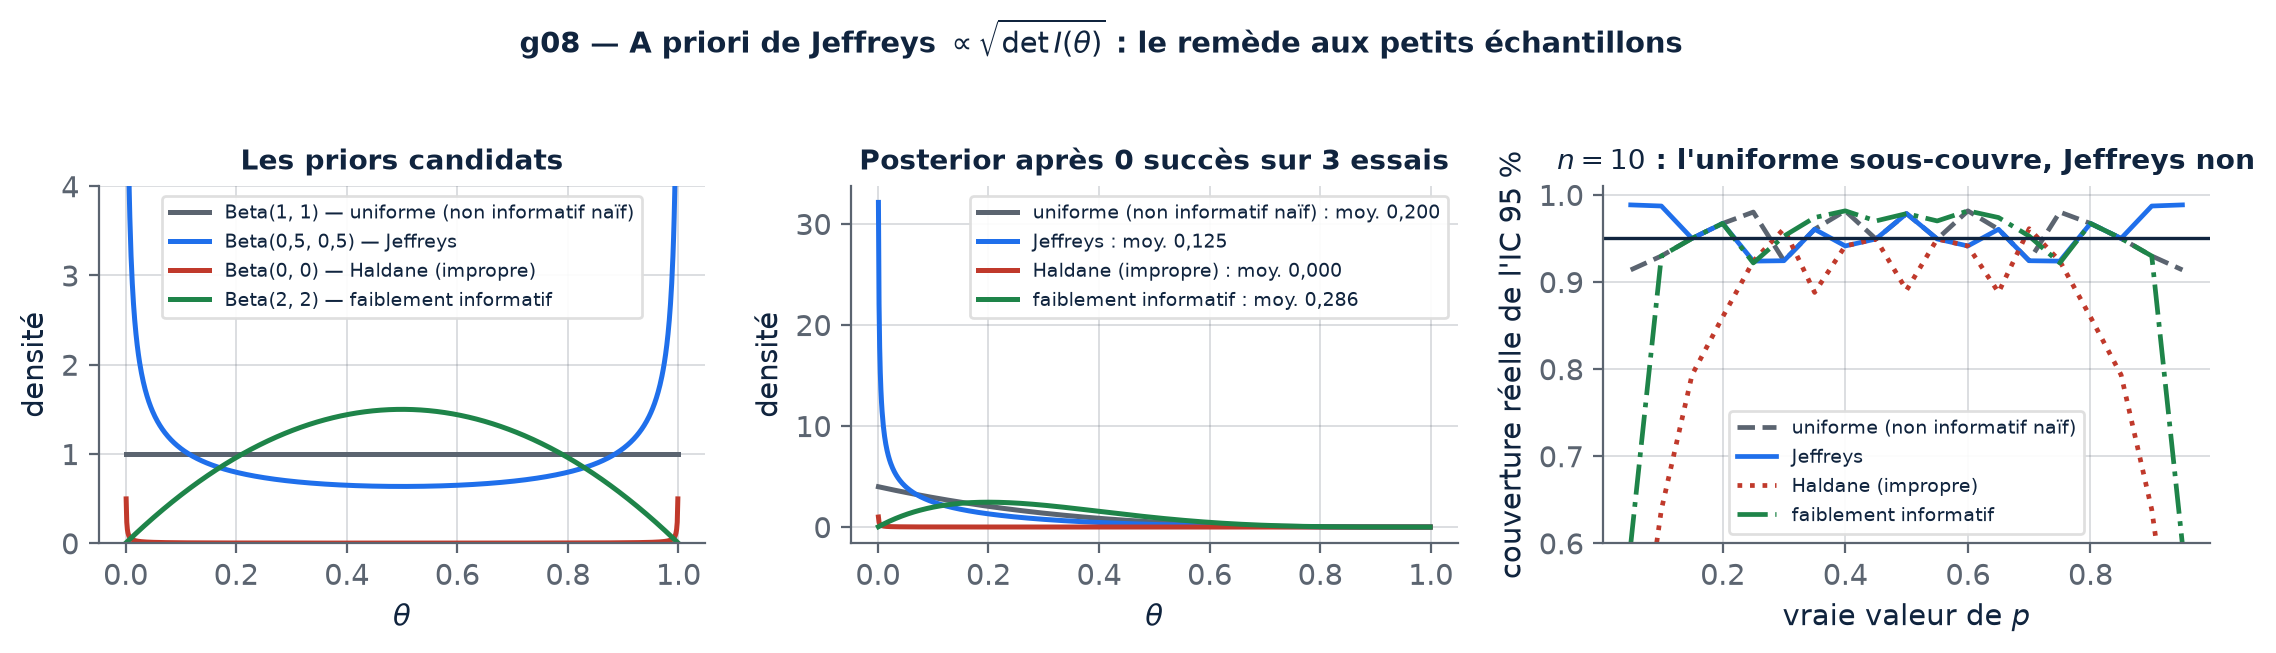
\includegraphics[width=0.90\textwidth]{g08_jeffreys.png}
\end{center}
\vspace{-4mm}
\begin{columns}[t]
\begin{column}{0.55\textwidth}
\begin{ebox}[Cas limite : $0$ succès sur $3$ essais]
\begin{tabular}{@{}lcc@{}}
\toprule
\textbf{Prior} & \textbf{moyenne} & \textbf{IC 95 \%} \\
\midrule
Uniforme Beta$(1,1)$ & 0,200 & $[0{,}0063 \,;\, 0{,}6024]$ \\
Jeffreys Beta$(0{,}5;0{,}5)$ & \textbf{0,125} & $[0{,}0002 \,;\, 0{,}5356]$ \\
Haldane Beta$(0,0)$ & 0,0003 & $[0{,}0000 \,;\, 0{,}0000]$ \\
Beta$(2,2)$ (faiblement inf.) & 0,2857 & $[0{,}0433 \,;\, 0{,}6412]$ \\
\bottomrule
\end{tabular}
\end{ebox}
\end{column}
\begin{column}{0.42\textwidth}
\begin{kbox}[La mesure qui départage]
Couverture réelle de l'IC 95 \% pour $n = 10$ (somme exacte sur les $2^{10}$
échantillons possibles) : uniforme $\in [0{,}914 ; 0{,}982]$, Jeffreys
$\in [0{,}924 ; 0{,}989]$, Beta$(2,2)$ $\in [0{,}599 ; 0{,}982]$.
Jeffreys est le plus \emph{honnête} aux valeurs extrêmes ; Haldane s'effondre
jusqu'à $0{,}390$.
\end{kbox}
\end{column}
\end{columns}
\end{frame}

% ---------------------------------------------------------------- 5
\begin{frame}{Propre contre impropre : la ligne rouge}
\begin{columns}[t]
\begin{column}{0.49\textwidth}
\begin{ebox}[Définitions]
Un prior est \textbf{propre} si $\int p(\theta)\,\mathrm{d}\theta = 1$.
Il est \textbf{impropre} si l'intégrale diverge, tout en restant utilisable
\emph{formellement} : l'uniforme sur $\R$, Beta$(0,0)$, $\mathrm{Gamma}(1/2,0)$,
$1/\sigma$.
\end{ebox}
\begin{solbox}[Ce qui se passe vraiment]
Un prior impropre est acceptable \textbf{si et seulement si} le posterior est
propre : c'est le cas de Haldane Beta$(0,0)$ face à $0$ succès sur $3$ essais
(posterior Beta$(0,3)$, moyenne $0{,}0003$), mais le posterior dégénère si
l'échantillon est vide ou si tous les succès sortent au même endroit.
\end{solbox}
\end{column}
\begin{column}{0.48\textwidth}
\begin{wbox}[Le mode d'échec qui ne prévient pas]
Avec un prior impropre et un posterior impropre, \textbf{aucun logiciel ne
plante} : PyMC échantillonne, les traces sont belles, les diagnostics sont verts,
et les intervalles sont faux. Il n'existe pas de test automatique.
\vspace{1mm}

Règle : vérifier \emph{à la main} que $\int p(y \given \theta) p(\theta)\mathrm{d}\theta < \infty$
avant de faire confiance à une sortie MCMC.
\end{wbox}
\begin{kbox}[Le compromis professionnel]
Impropre pour \emph{démarrer} (Jeffreys, référence) ; propre pour
\emph{publier} : on montre que le posterior est stable quand on tronque le prior
sur un domaine fini.
\end{kbox}
\end{column}
\end{columns}
\end{frame}

% ---------------------------------------------------------------- 6
% [split]
\begin{frame}{La subtilité du prior uniforme sur un paramètre d'échelle}
\begin{center}
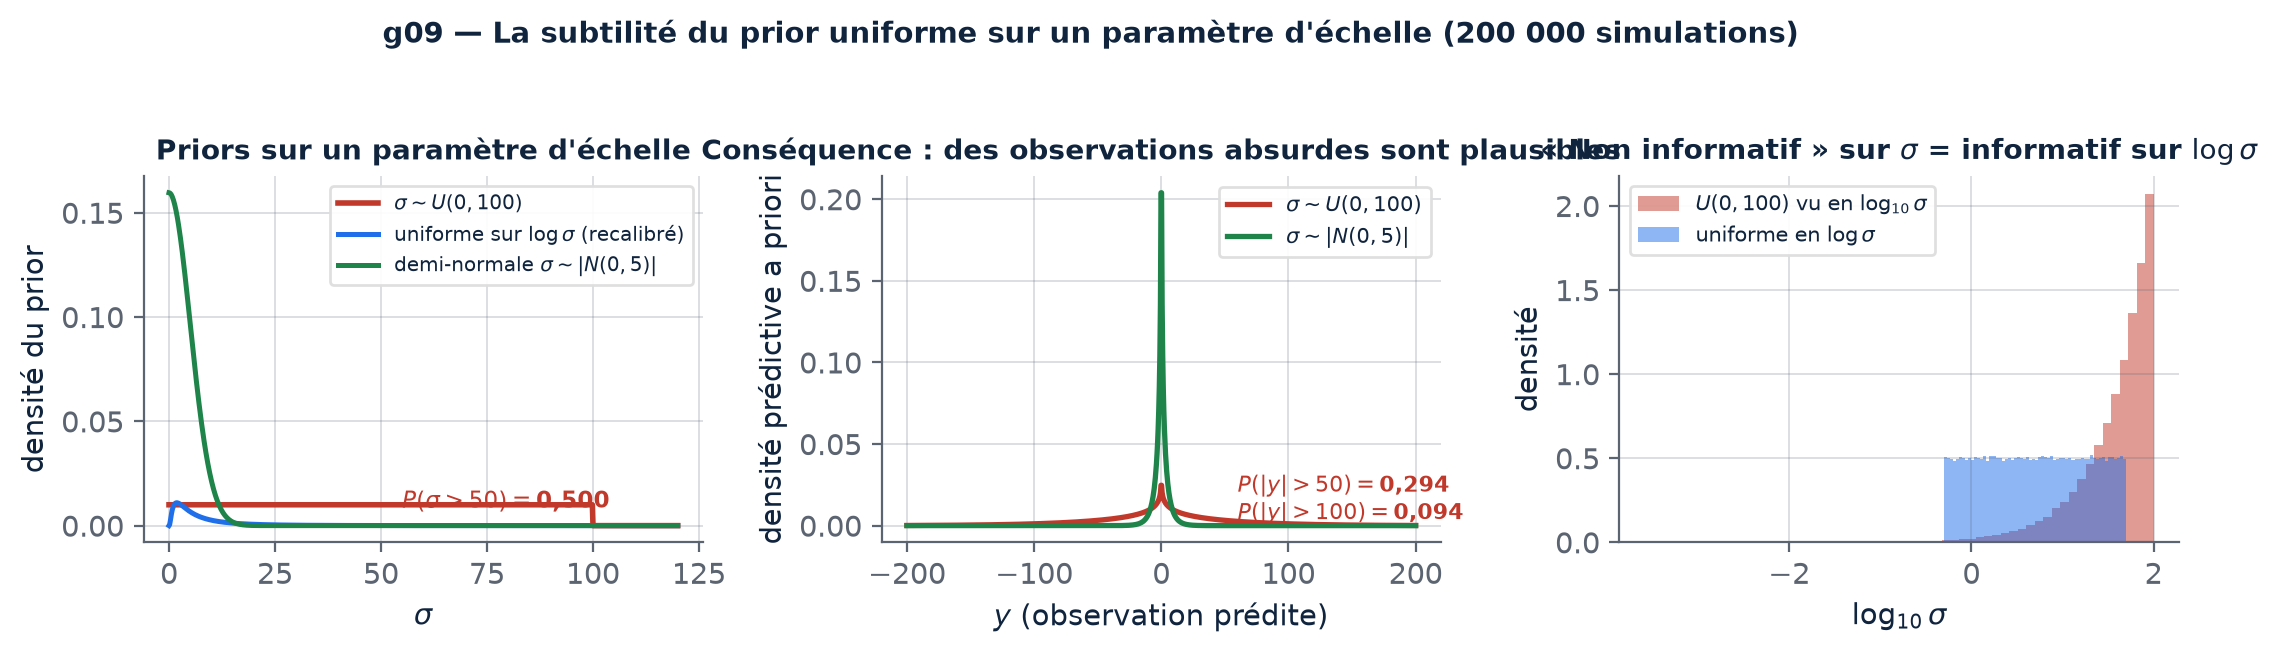
\includegraphics[width=.86\textwidth]{g09_uniforme_echelle.png}
\end{center}
\end{frame}

% [split]
% [suite]
\begin{frame}{La subtilité du prior uniforme sur un paramètre d'échelle}
\vspace{-1mm}
\begin{columns}[t]
\begin{column}{0.55\textwidth}
\begin{ebox}[Ce que disent les simulations]
Avec $\sigma \sim U(0, 100)$ (a priori « je n'en sais rien ») :
$P(\sigma > 50) = 0{,}500$ et la médiane de $\sigma$ vaut $50$.
Conséquence sur une observation $y \sim \N(0,\sigma)$ :
$P(|y| > 50) = 0{,}294$ et $P(|y| > 100) = 0{,}094$.
Un modèle de points SAT prédit donc des effets de $+100$ points comme
un événement banal.
\end{ebox}
\end{column}
\begin{column}{0.40\textwidth}
\begin{wbox}[L'erreur d'interprétation]
« Non informatif » sur $\sigma$ \textbf{devient très informatif} sur
$\log\sigma$ : la figure de droite montre la masse concentrée vers les grandes
valeurs. En informatique numérique on travaille presque toujours avec
$\log\sigma$ — donc un prior uniforme sur $\sigma$ n'est pas neutre du point
de vue de l'échelle, celui qui compte vraiment.
\end{wbox}
\end{column}
\end{columns}
\end{frame}

% [suite]
\begin{frame}{La subtilité du prior uniforme sur un paramètre d'échelle (suite)}
\begin{kbox}[La solution recommandée]
Un a priori uniforme sur $\log\sigma$, ou une demi-normale faiblement
informative (échelle fixée par la connaissance du phénomène), et
\textbf{toujours un contrôle prédictif a priori} avant de conclure.
\end{kbox}

\end{frame}

% ---------------------------------------------------------------- 7
% [suite]
\begin{frame}{L'a priori faiblement informatif : la voie raisonnable}
\begin{kbox}[Le principe de la standardisation]
Avant de choisir une échelle, on \textbf{standardise} : on exprime le paramètre en
unités de la variabilité du phénomène.
\[
z = \frac{y - \bar y}{s_y}, \qquad \text{puis } z \sim \N(0, 1) \text{ a priori}
\]
Le même prior marche alors pour des données en points SAT, en euros ou en secondes.
\end{kbox}
\vspace{1mm}
\begin{columns}[t]
\begin{column}{0.52\textwidth}
\begin{ebox}[Application aux 8 écoles]
Effets estimés en points SAT : moyenne $\mathbf{8{,}820}$,
écart-type $s_y = \mathbf{10{,}514}$, étendue $[-2{,}75 \,;\, 28{,}39]$,
erreur standard moyenne $12{,}650$.
Variables standardisées : $\mathbf{1{,}861}$, $\mathbf{-0{,}084}$,
$\mathbf{0{,}874}$, $\mathbf{0{,}318}$ pour les écoles A, B, G, H.
\end{ebox}
\end{column}
\begin{column}{0.45\textwidth}
\begin{ebox}[Traduire un dire d'expert]
« L'effet est faiblement positif, peut-être 10 points, sûrement pas
100 » se traduit par
$\mu \sim \N(10, 20^2)$, ou bien, en unités standardisées, $\mu \sim \N(0{,}5, 1^2)$ sur $z$.
puis on vérifie ce que ce prior prédit (section 2.3).
\end{ebox}
\end{column}
\end{columns}
\vspace{1mm}
\end{frame}

% [suite]
\begin{frame}{L'a priori faiblement informatif : la voie raisonnable (suite)}
\begin{wbox}[Pourquoi « faiblement informatif »]
Un prior faiblement informatif \textbf{régularise} les situations dégénérées
(une catégorie sans observation, une séparation parfaite en régression) tout en
laissant les données décider. C'est le réglage par défaut d'une analyse sérieuse.
\end{wbox}
\end{frame}

% ---------------------------------------------------------------- 8
\begin{frame}{Quiz 2 — choisir un a priori}
% [rogna]
\small
\begin{qbox}[Question 4 -- Classer et justifier]
\textbf{1.} Un capteur mesure un taux $\lambda$ de défauts par pièce. La chaîne
produit de 1 à 50 pièces par heure. Quel prior est préférable pour l'échelle :
$U(0, 100)$ sur $\lambda$, ou $U(\log \lambda)$, ou $\mathrm{Gamma}(1,1)$ ? \\[1mm]
\textbf{2.} Un collègue affirme : « j'ai mis $\mathrm{Beta}(1,1)$, donc mon
posterior est objectif ». Que répondez-vous ? \\[1mm]
\textbf{3.} Pour une proportion, $10$ essais antérieurs donnent $3$ succès.
Écrire un a priori faiblement informatif qui ne les ignore pas \emph{et} ne les
impose pas. \\[1mm]
\textbf{4.} Le tableau de la frame « boîte à outils » donne Beta$(0{,}5;0{,}5)$
comme impropre : comment est-ce possible pour la loi de Jeffreys de la
\emph{binomiale} ? \\[1mm]
\textbf{5.} Un paramètre d'échelle $\sigma$ est contraint physiquement :
$0 < \sigma < 200$. Quelle famille choisir, et laquelle éviter ?
\vspace{1.5mm}

\textcolor{byBlue}{\textbf{Éléments de réponse :}}
\textbf{1.} $U(\log\lambda)$ ou Gamma (invariance d'échelle) ;
un $U(0,100)$ donne la moitié de sa masse à $\lambda > 50$ : absurde.
\quad
\textbf{2.} Que l'uniforme \emph{n'est pas} invariant : il devient très informatif
après reparamétrisation.
\quad
\textbf{3.} Beta$(1+3a, 1+7a)$ avec $a = 0{,}5$ : Beta$(2{,}5; 4{,}5)$, soit un poids
de $50$ \% pour l'historique.
\quad
\textbf{4.} Impropre \emph{a priori}, propre \emph{a posteriori} : les observations
apportent la convergence.
\quad
\textbf{5.} Une demi-normale tronquée ou une log-uniforme ; éviter le mélange
uniforme sur $\sigma$ qui favorise les grandes valeurs.
\end{qbox}
\end{frame}

% ---------------------------------------------------------------- 9
% [suite]
\begin{frame}{Activité guidée — éliciter un a priori (10 min)}
% [rogna]
\small
\begin{abox}[Consigne, par binôme de rôles]
L'énoncé de l'expert : « \emph{Le taux de retour d'un produit est faible, autour de
2 \%, je dirais entre 0,5 \% et 5 \%. Je n'ai jamais vu plus de 10 \%.} »
\begin{enumerate}
  \item Proposer une loi a priori, justifier la famille et les hyperparamètres.
  \item Calculer $a+b$ et commenter le nombre d'observations virtuelles.
  \item Vérifier par un contrôle prédictif quel nombre de retours ce prior prédit
        sur une commande de $200$ pièces.
\end{enumerate}
\end{abox}
\vspace{1mm}
\end{frame}

% [suite]
\begin{frame}{Activité guidée — éliciter un a priori (10 min) (suite)}
\begin{columns}[t]
\begin{column}{0.54\textwidth}
\begin{solbox}[Une réponse parmi d'autres (calculée)]
$\mathrm{Beta}(a,b)$ centré en $0{,}02$ avec $P(p < 0{,}05) \approx 0{,}95$ :
Beta$(2, 98)$ — moyenne $0{,}0200$, $a+b = 100$ soit
\textbf{98 observations virtuelles}, IC 95 \% $[0{,}0025 \,;\, 0{,}0550]$,
et $P(p < 0{,}05) = 0{,}9613$.
Sur $200$ pièces, le contrôle prédictif (20\,000 simulations) donne en moyenne
$3{,}99$ retours, un intervalle à $90$ \% de $[0 \,;\, 11]$ et
$P(k > 20) = 0{,}0011$ : le prior n'annonce jamais de catastrophes.
\end{solbox}
\end{column}
\begin{column}{0.43\textwidth}
\begin{ebox}[Un bon exercice d'ingénierie]
\begin{itemize}
  \item On a transformé une phrase en \textbf{deux nombres vérifiables} ;
  \item l'expert peut \emph{réfuter} : « 98 observations virtuelles, c'est
        trop, je ne suis pas si sûr » ;
  \item le désaccord devient un paramètre ($a+b$), donc une analyse de sensibilité
        (section 2.4) plutôt qu'une discussion de couloir.
\end{itemize}
\end{ebox}
\end{column}
\end{columns}
\end{frame}

% ---------------------------------------------------------------- 10
% [suite]
\begin{frame}{2.3 — Simuler avant d'avoir des données}
\begin{kbox}[L'idée en une phrase]
Avant d'estimer quoi que ce soit, on \textbf{simule le monde que le modèle
promet} — paramètres tirés du prior, puis données tirées de la vraisemblance — et
on se demande : ces données ressemblent-elles à celles qu'on \emph{attend} ?
\end{kbox}
\vspace{1mm}
\begin{columns}[t]
\begin{column}{0.50\textwidth}
\begin{ebox}[Un examen du prior]
Un \emph{prior predictive check} (PPC) ne regarde jamais les observations réelles
pour ajuster : il vérifie que le \textbf{domaine de plausibilité} du modèle est
compatible avec la physique ou le bon sens. C'est l'étape qui aurait sauvé
des projets entiers de deep learning bayésien.
\end{ebox}
\end{column}
\begin{column}{0.47\textwidth}
\begin{abox}[À faire devant la classe (2 min)]
Reprendre l'énoncé de l'expert de la frame précédente : avant même de collecter
des données, combien de retours le modèle peut-il prédire sur 200 pièces ?
Si la réponse dépasse 40, le prior est intenable.
\end{abox}
\end{column}
\end{columns}
\vspace{1mm}
\end{frame}

% [suite]
\begin{frame}{2.3 — Simuler avant d'avoir des données (suite)}
\begin{tcolorbox}[colback=byCyan!8,colframe=byCyan,arc=2mm,width=.95\textwidth]
\small\centering
\textbf{Ordre de travail professionnel} : (1) écrire le modèle, (2) simuler le prior
prédictif, (3) corriger l'échelle, (4) seulement alors regarder les données,
(5) vérifier le posterior prédictif (chapitres 3 et 4).
\end{tcolorbox}
\end{frame}

% ---------------------------------------------------------------- 11
\begin{frame}{Le contrôle prédictif a priori, en quatre étapes}
\begin{ebox}[La loi prédictive a priori]
\[
p(\tilde y) = \int p(\tilde y \given \theta)\, p(\theta)\,\mathrm{d}\theta
\qquad \text{simulation : } \theta^{(s)} \sim p(\theta),\;\;
\tilde y^{(s)} \sim p(\tilde y \given \theta^{(s)})
\]
\begin{enumerate}
  \item \textbf{Tirer} $S$ valeurs du paramètre sous le prior
        ($S = 20\,000$ dans nos scripts, $4\,000$ en PyMC).
  \item \textbf{Propager} dans la vraisemblance : on obtient $S$ jeux de données simulés.
  \item \textbf{Résumer} : moyenne prédite, intervalle à 90 \%, probabilité d'événements impossibles.
  \item \textbf{Juger} : ce que le modèle promet est-il physiquement admissible ?
        Sinon, recommencer à l'étape 1 avec une échelle corrigée.
\end{enumerate}
\end{ebox}
\vspace{1mm}
\begin{kbox}[Ce que l'étape 4 ne doit jamais être]
Un test statistique automatique. Le jugement est \textbf{métier} : « une teneur en
sucre négative », « une probabilité de 1,0 », « un effet de 300 points SAT ».
Le graphique remplace le test.
\end{kbox}
\end{frame}

% ---------------------------------------------------------------- 12
% [rogna]
% [rogna]
% [rogna]
% [split]
\begin{frame}{Que prédit chaque a priori ? Le cas Challenger}
\begin{center}
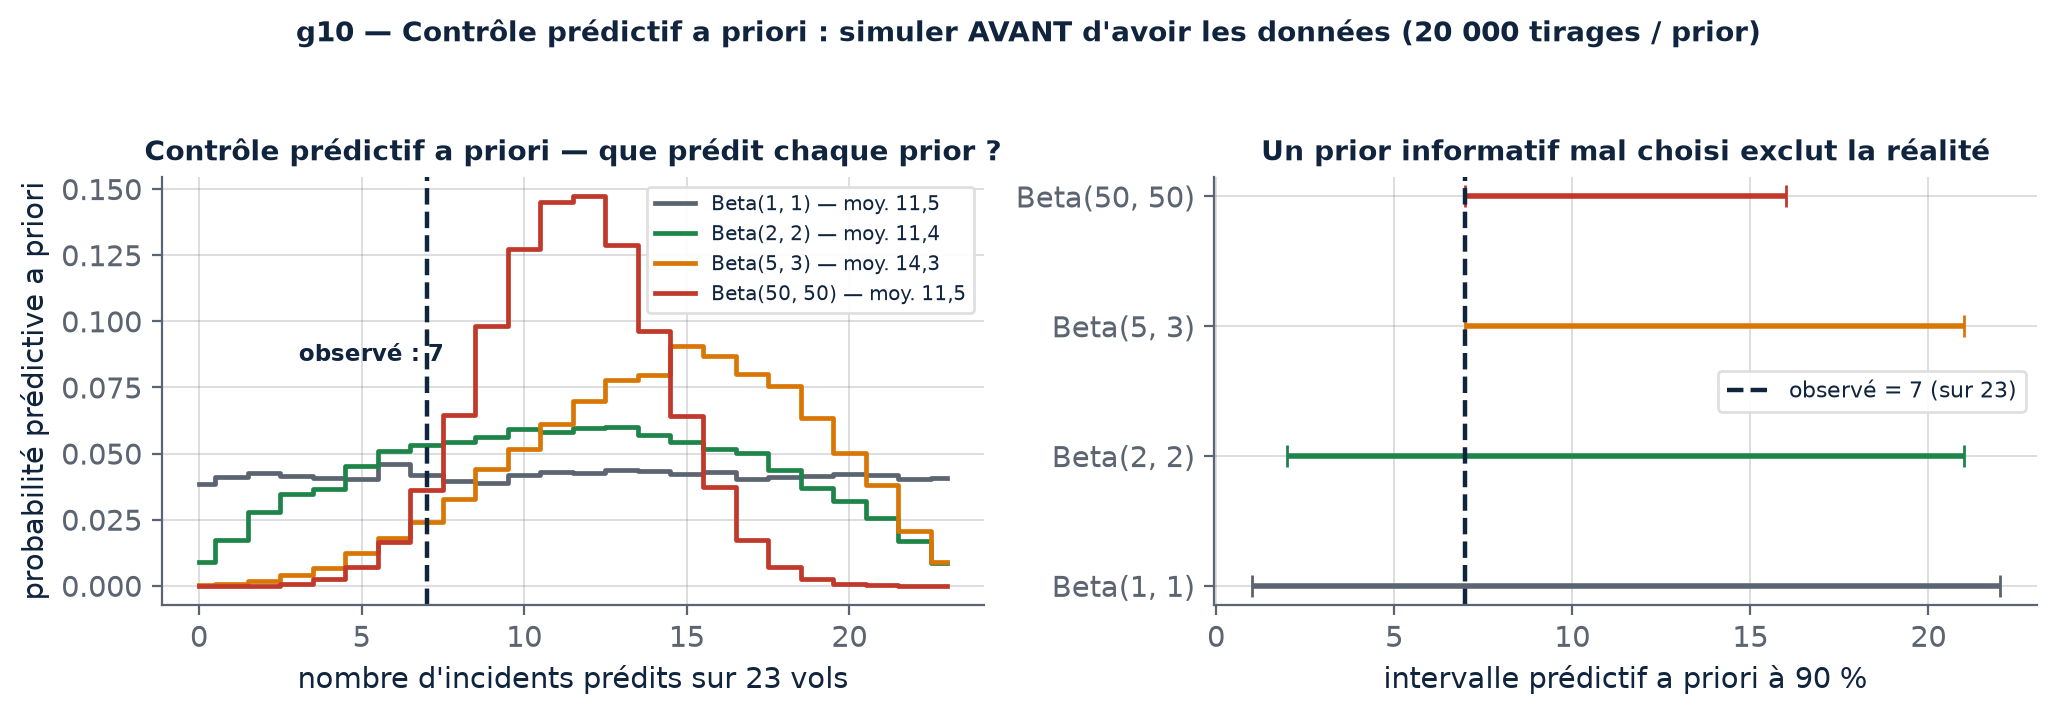
\includegraphics[width=.86\textwidth]{g10_prior_predictive.png}
\end{center}
\end{frame}

% [split]
\begin{frame}{Que prédit chaque a priori ? Le cas Challenger}

\vspace{-1mm}
\centering
\scriptsize\begin{tabular}{@{}lcccc@{}}
\toprule
\textbf{A priori} & \textbf{nombre prédit} & \textbf{intervalle 90 \%} &
$P(k \leq 7)$ & $P(p > 0{,}5)$ \\
\midrule
Beta$(1,1)$ & 11,52 & $[1 \,;\, 22]$ & $0{,}333$ & $0{,}499$ \\
Beta$(2,2)$ & 11,43 & $[2 \,;\, 21]$ & $0{,}275$ & $0{,}502$ \\
Beta$(5,3)$ & 14,35 & $[7 \,;\, 21]$ & $0{,}068$ & \textbf{0,769} \\
Beta$(50,50)$ & 11,51 & $[7 \,;\, 16]$ & $0{,}063$ & $0{,}504$ \\
\bottomrule
\end{tabular}
\vspace{1.5mm}

\begin{minipage}{.95\textwidth}
\begin{wbox}[Le verdict du contrôle]
Les valeurs réellement observées : $k = 7$ incidents sur $23$ vols.
Elle est 	extbf{parfaitement plausible} sous Beta$(1,1)$ (33	extsuperscript{e} percentile)
et 	extbf{très improbable} sous Beta$(5,3)$ et Beta$(50,50)$ (quantiles $0{,}068$ et
$0{,}063$). Conclusion : un prior centré sur 0,5 (le taux attendu d'une
pièce équilibrée) aurait \emph{exclu la réalité} — c'est exactement le diagnostic
que le PPC doit produire avant l'analyse.
\end{wbox}
\end{minipage}
\end{frame}

% ---------------------------------------------------------------- 13
% [rogna]
% [rogna]
% [rogna]
% [split]
\begin{frame}{Calibrer l'échelle : le cas d'école des huit écoles}
\begin{center}
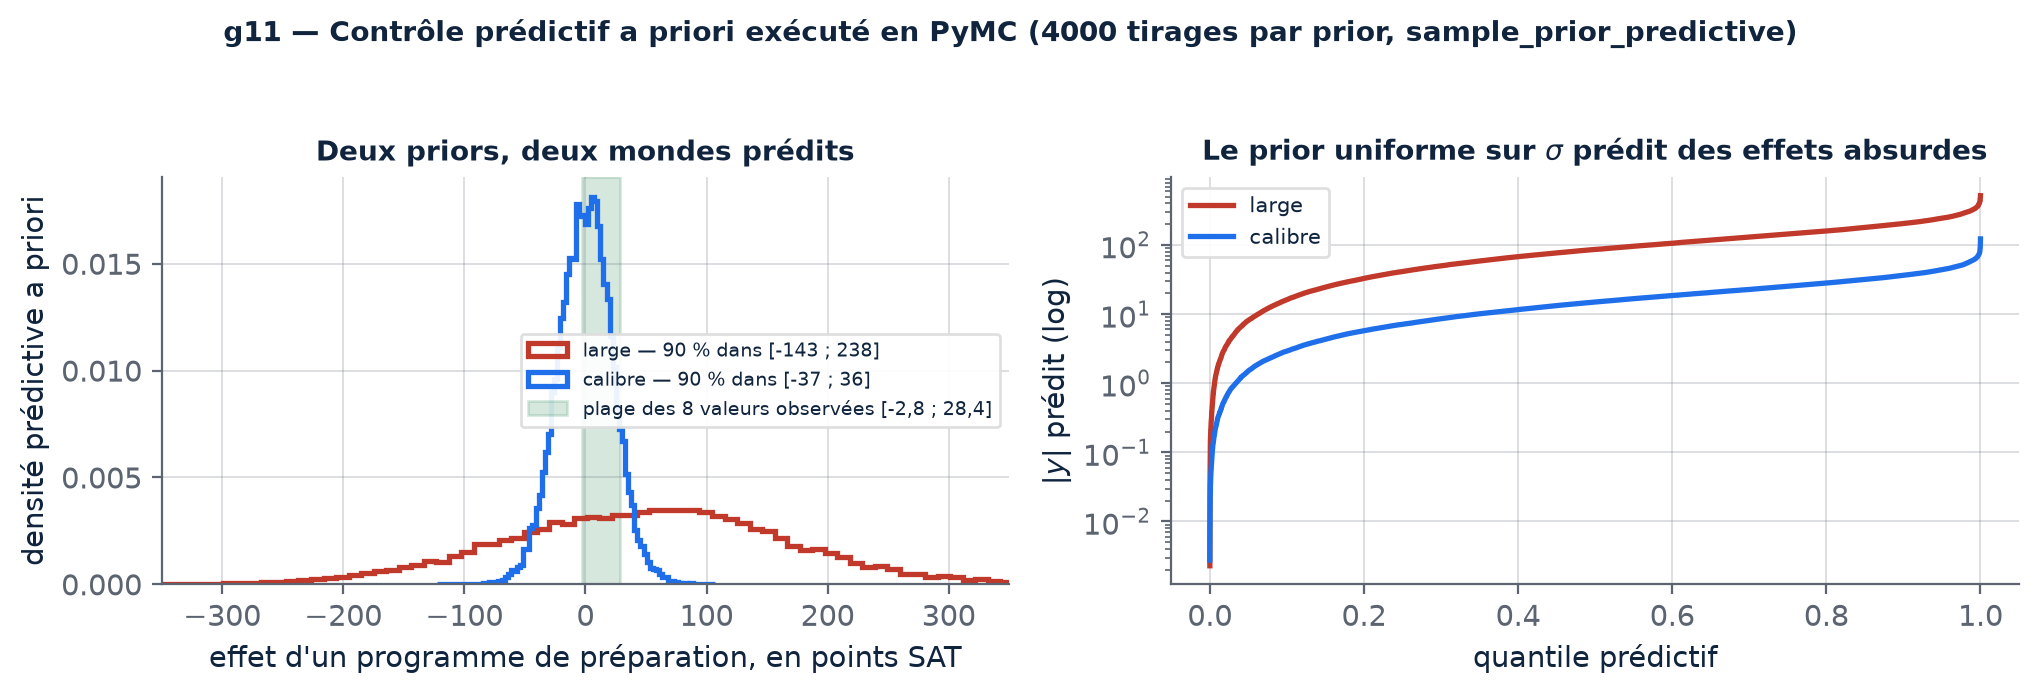
\includegraphics[width=.86\textwidth]{g11_prior_predictive_pymc.png}
\end{center}
\end{frame}

% [split]
\begin{frame}{Calibrer l'échelle : le cas d'école des huit écoles}

\vspace{-1mm}
\begin{columns}[t]
\begin{column}{0.55\textwidth}
\begin{ebox}[Deux priors exécutés en PyMC]
Effets attendus d'un programme SAT, en points ; les valeurs observées vivent
dans $[-2{,}75 \,;\, 28{,}39]$.
\begin{itemize}
  \item prior \textbf{calibré} : $\mu \sim \N(0, 20^2)$, $\sigma \sim \mathrm{HN}(10)$
        $\Rightarrow$ 90 \% des effets prédits dans $[-37{,}0 \,;\, 36{,}0]$ points, et
        seulement $0{,}02$ \% des cas au-delà de $\pm 100$ points : compatible avec la réalité ;
  \item prior \textbf{large} : $\mu \sim \N(50, 100^2)$, $\sigma \sim U(0,100)$
        $\Rightarrow$ 90 \% des effets dans $[-142{,}7 \,;\, 238{,}2]$, amplitudes
        de $\pm 324{,}9$ points au 99\textsuperscript{e} percentile et
        $P(|y| > 100) = \mathbf{0{,}430}$ : quatre effets prédits sur dix sont
        absurdes pour un test scolaire.
\end{itemize}
\end{ebox}
\end{column}
\begin{column}{0.42\textwidth}
\begin{kbox}[Le réflexe]
Le contrôle prédictif a priori ne sert pas à \emph{choisir} entre deux théories :
il sert à \textbf{éliminer les échelles impossibles}, puis à retenir une échelle
faiblement informative qui laisse les données décider.
\end{kbox}
\end{column}
\end{columns}
\end{frame}

% ---------------------------------------------------------------- 14
% [suite5]
\begin{frame}[fragile]{La ligne de code qui change une analyse}
\begin{columns}[t]
\begin{column}{0.54\textwidth}
\begin{codebox}[src/fig\_ch2b\_pymc.py — PPC sur le modèle des 8 écoles]
\begin{lstlisting}
y = np.array([28.39, 7.94, -2.75, 6.82,
              -0.64, 0.63, 18.01, 12.16])

with pm.Model() as m:
    mu = pm.Normal("mu", mu=0, sigma=20)     # calibre
    sigma = pm.HalfNormal("sigma", 10)
    pm.Normal("y", mu=mu, sigma=sigma, shape=8)

    # 4000 mondes possibles AVANT toute donnee
    prior = pm.sample_prior_predictive(draws=4000,
                                       random_seed=42)

ypred = prior.prior["y"].values.reshape(-1, 8)
print(np.percentile(ypred, [5, 50, 95]))
print((np.abs(ypred) > 100).mean())

# puis seulement : pm.sample() pour le posterior
\end{lstlisting}
\end{codebox}
\end{column}
\begin{column}{0.43\textwidth}
\begin{kbox}[Trois bonnes pratiques de code]
\begin{itemize}
  \item Un \textbf{script par question} : le PPC dans le fichier du modèle ;
  \item une \py{random_seed} fixée : un contrôle doit être reproductible ;
  \item sauvegarder les chiffres (ici \file{figures/key\_numbers\_ch2.json})
        pour que les slides citent des valeurs exécutées.
\end{itemize}
\end{kbox}
\end{column}
\end{columns}
\end{frame}

% [suite5]
\begin{frame}{La ligne de code qui change une analyse (suite)}
\begin{wbox}[Le piège de la relecture]
\py{sample_prior_predictive} place ses tirages dans le groupe \py{prior} de
l'objet ArviZ (et non dans \py{prior_predictive}) : vérifier le nom du groupe
— c'est l'erreur qui a réellement interrompu ce script à la première exécution.
\end{wbox}
\end{frame}

% ---------------------------------------------------------------- 15
\begin{frame}{Du contrôle a priori au contrôle a posteriori}
\begin{columns}[t]
\begin{column}{0.49\textwidth}
\begin{kbox}[Prior predictive check (PPC)]
\begin{itemize}
  \item \textbf{Quand} : avant de voir les données.
  \item \textbf{Distribution} : $p(\tilde y) = \int p(\tilde y \given \theta)p(\theta)\mathrm{d}\theta$.
  \item \textbf{Question} : le modèle prédit-il un monde possible ?
  \item \textbf{Décision} : corriger l'échelle du prior.
\end{itemize}
\end{kbox}
\end{column}
\begin{column}{0.49\textwidth}
\begin{kbox}[Posterior predictive check (PPC$'$)]
\begin{itemize}
  \item \textbf{Quand} : après l'inférence.
  \item \textbf{Distribution} : $p(\tilde y \given y) = \int p(\tilde y \given \theta)p(\theta \given y)\mathrm{d}\theta$.
  \item \textbf{Question} : le modèle \emph{ajusté} reproduit-il les données ?
  \item \textbf{Décision} : revoir le modèle (chapitres 3 et 4).
\end{itemize}
\end{kbox}
\end{column}
\end{columns}
\vspace{1mm}
\begin{ebox}[Les deux contrôles de ce cours]
Sur Challenger, le contrôle a priori compare les 4 priors du paragraphe précédent
(bonnes échelles) ; sur les 8 écoles, le contrôle a posteriori du chapitre 3 vérifie
que les effets simulés couvrent bien les 8 effets observés. Un modèle qui passe les
deux est un modèle \textbf{crédible}, pas seulement convergé.
\end{ebox}
\end{frame}

% ---------------------------------------------------------------- 16
\begin{frame}{Pièges du contrôle prédictif}
\begin{qbox}[Question 5 -- Le PPC trompeur]
Un étudiant annonce : « mon PPC est parfait : les données simulées couvrent exactement
les données observées ».
\vspace{1mm}

\textbf{a)} Qu'a-t-il probablement fait de mal ? \\[1mm]
\textbf{b)} Peut-on \emph{valider} un modèle avec un PPC ? \\[1mm]
\textbf{c)} Un prior tellement large que tout est prédit doit-il être préféré ?
\vspace{1.5mm}

\textcolor{byBlue}{\textbf{Réponses :}}
\textbf{a)} Un prior trop large prédit tout : la couverture ne coûte rien.
Il faut regarder aussi la \emph{concentration} des prédictions
(ici, un intervalle à 90 \% de 22 valeurs pour $n=23$ ne discrimine rien).
\quad
\textbf{b)} Non : un PPC ne \emph{falsifie} que des modèles grossièrement faux ;
il n'établit jamais la vérité d'un modèle — seule la prévision hors échantillon
répond à cette question.
\quad
\textbf{c)} Non : un prior qui prédit un taux d'incident de 95 \% est plus
« couvrant » et pourtant inutilisable ; le but est la \emph{calibration}, pas la
largeur.
\end{qbox}
\end{frame}

% ---------------------------------------------------------------- 17
\begin{frame}{Synthèse 2.2 et 2.3 — choisir et tester son a priori}
% [rogna]
\small
\begin{kbox}[Six règles issues de la pratique]
\begin{enumerate}
  \item Écrire le prior en \textbf{taille d'échantillon virtuelle} ($a+b$, $n_0$) et
        le dire à voix haute.
  \item Préférer un a priori \textbf{faiblement informatif} sur une échelle
        standardisée ; réserver le non informatif à un objectif d'invariance
        affiché.
  \item Sur un paramètre d'échelle, \textbf{jamais} d'uniforme sur $\sigma$ :
        travailler sur $\log\sigma$ ou avec une demi-normale calibrée.
  \item Vérifier la \textbf{propreté} du posterior quand le prior est impropre.
  \item Faire un \textbf{contrôle prédictif a priori} et savoir citer au moins un
        événement prédit impossible.
  \item Documenter : modèle, prior, échelle, contrôle — dans le rapport, pas dans
        les commentaires du code.
\end{enumerate}
\end{kbox}
\vspace{-2mm}
\begin{columns}[t]
\begin{column}{0.55\textwidth}
\begin{ebox}[Transition vers 2.4]
Il reste la question la plus redoutée : « et si je change d'avis sur le prior ? »
La section suivante quantifie la \textbf{sensibilité} et la rend mesurable.
\end{ebox}
\end{column}
\begin{column}{0.42\textwidth}
\begin{wbox}[Les trois chiffres à retenir]
Beta$(50,50)$ face à 23 données : $w = 0{,}813$ \; ; \; uniforme sur $\sigma$ :
$P(|y| > 100) = 0{,}094$ \; ; \; Beta$(5,3)$ exclut la réalité observée au seuil de
$7$ \%.
\end{wbox}
\end{column}
\end{columns}
\end{frame}
